\subsection{Canvas}
\hspace{0.55cm}La etiqueta \textbf{canvas} es un contenedor para figuras o gráficos un poco más especializados o complejos, a diferencia de \textit{svg}, es necesario un script (JavaScript suele ser utilizado) para dibujar dentro de este contenedor.
\begin{center}
    \textit{$<$canvas id="canvas1" width="200" height="200"$>$$<$canvas$/>$}
\end{center}

El atributo \textit{id} se hace presente, porque es necesario para pasárselo al script, que le regresará un gráfico al contenedor canvas:
\begin{lstlisting}
    <!-- Crea un panel de dibujo Canvas de 400x300 píxeles. -->
    <canvas id="canvas1" width="400" height="300"></canvas> 

    <script>
        // Asigna a una variable el contenedor con id "canvas1".
        var can = document.getElementById("canvas1"); 
        // Establece el tipo de dibujo en 2D.
        var ctx = can.getContext("2d");
    </script>
\end{lstlisting}

Al igual que en svg, las coordenadas que maneja canvas son \textit{x}, \textit{y}, cada una de ellas empujan el gráfico insertado igual que como ocurre en svg (de izquierda a derecha y de superior a inferior en la página). Al igual que con svg, existen métodos de JS para dibujar figuras y pasárselos al canvas.

El método \textbf{fillRect(x, y, w, h)} dibuja un cuadrado o rectángulo rellenado (obligado) de color negro (por defecto), podemos suponer que los parámetros representan las coordenadas y dimensiones de la figura respectivamente. Pongamos un ejemplo y su resultado (\textit{Figura \ref{fig: 27}}):
\begin{lstlisting}
    <canvas id="canvas1" width="900" height="900"></canvas>
        
    <script>
        var c=document.getElementById("canvas1");
        var ctx=c.getContext("2d");
        // Dibuja un cuadrado con origen en (30,30) de 200x200 píxeles.
        ctx.fillRect(30,30,200,200);
    </script>
\end{lstlisting}
\begin{figure}[H]
    \centering
    \caption{Dibujando un cuadrado con Canvas}
    \label{fig: 27}
    
\includegraphics[width=7cm]{ss_html/canvas.png}
\end{figure}

Existen algunos otros métodos para personalizar y crear gráficos:
\begin{itemize}
    \item \textbf{fillStyle}: establece color, degradado o patrón de rellenado para el gráfico.
    \item \textbf{moveTo(x,y)}: define el punto inicial para dibujar una línea.
    \item \textbf{lineTo(x,y)}: define el punto terminal para dibujar una línea.
    \item \textbf{beginPath()}: establece el modo para dibujar un círculo.
    \item \textbf{arc(x,y,r,comienzo,fin)}: establece los parámetros para dibujar un círculo.
    \item \textbf{stroke()}: dibuja un círculo.
    \item \textbf{createLinearGradient(x,y,x1,y2)}: crea un degradado lineal.
    \item \textbf{createRadialGradient(x,y,r,x1,y1,r1)}: crea un degradado circular.
    \item \textbf{font}: establece la letra, formato y tamaño del texto a dibujar.
    \item \textbf{fillText(texto,x,y)}: dibuja un texto rellenado.
    \item \textbf{strokeText(texto,x,y)}: dibuja un texto no rellenado.
    \item Entre otros.
\end{itemize}


\subsubsection{Transformaciones Canvas}
\hspace{0.55cm}Un gráfico Canvas puede ser transformado una vez este fue creado, el método \textbf{translate(x,y)} mueve un gráfico a otra posición: \textbf{x} representa la distancia horizontal que se moverá el gráfico, \textbf{y} representa la distancia vertical que se moverá. La \textit{Figura \ref{fig: 28}} muestra el resultado de un ejemplo de esta función:
\begin{lstlisting}
    <canvas id="canvas1" width="400" height="300"></canvas> 
            
    <script>
        var c=document.getElementById("canvas1");
        var ctx=c.getContext("2d");
        // Establece el estilo, tamaño y tipografia del texto.
        ctx.font="bold 22px Tahoma";
        // Establece la alineación del texto.
        ctx.textAlign="start";
        // Posición original.
        ctx.fillText("start", 10, 30);
        // Posición para transformación.
        ctx.translate(100, 150);
        ctx.fillText("after translate", 10, 30);
    </script>
\end{lstlisting}
\begin{figure}[H]
    \centering
    \caption{Trasladando una gráfico con Canvas}
    \label{fig: 28}
    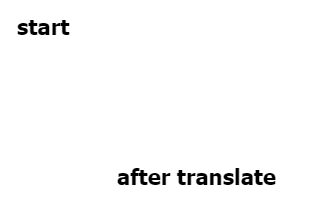
\includegraphics[width=5cm]{ss_html/canvas_translate.png}
\end{figure}

El método \textbf{rotate()} rota un gráfico. Los valores que acepte este método deben estar en \textbf{radianes}, no grados. La \textit{Figura \ref{fig: 29}} muestra el resultado de un ejemplo de esta función:
\begin{lstlisting}
    <canvas id="canvas1" width="900" height="900"></canvas> 
            
    <script>
        var c=document.getElementById("canvas1");
        var ctx=c.getContext("2d");
        // Aspecto del cuadrado antes de la rotación.
        ctx.fillStyle = "#FF0000";
        ctx.fillRect(150,60,200,200);
        // Rotación de la figura.
        ctx.rotate((Math.PI / 180) * 25);  // Rota 25 grados.
        // Aspecto del cuadrado después de la rotación.
        ctx.fillStyle = "#0000FF";
        ctx.fillRect(150,60,200,200);
    </script>
\end{lstlisting}
\begin{figure}[H]
    \centering
    \caption{Rotando una gráfico con Canvas}
    \label{fig: 29}
    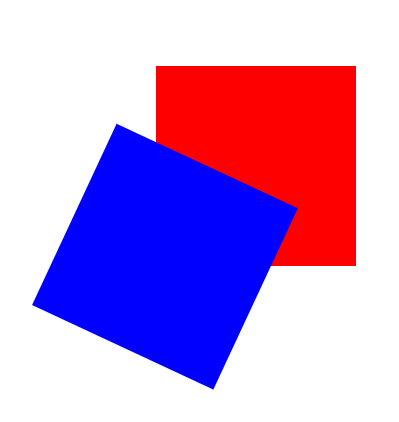
\includegraphics[width=7cm]{ss_html/canvas_rotate.png}
\end{figure}

El método \textbf{scale(x, y)} escala un gráfico, el parámetro \textit{x} indica la cantidad de veces que el gráfico será escalado en la dirección x, mientras que el parámetro \textit{y} indica la cantidad de veces que el gráfico será escalado en la dirección y. La \textit{Figura \ref{fig: 30}} muestra el resultado de un ejemplo de esta función:
\begin{lstlisting}
    <canvas id="canvas1" width="900" height="900"></canvas> 
            
    <script>
        var c=document.getElementById("canvas1");
        var ctx=c.getContext("2d");
        ctx.font="bold 22px Tahoma";
        ctx.textAlign="start";
        // Aspecto del texto en una ubicación.
        ctx.fillText("start", 10, 30);
        
        ctx.scale(1.5, 4);  // Escala el texto 1.5 veces en el eje X y 4 veces en el eje Y.

        // Mantiene el texto, pero lo ubica en otro sitio.
        ctx.fillText("start", 10, 60);
    </script>
\end{lstlisting}
\begin{figure}[H]
    \centering
    \caption{Escalando un gráfico con Canvas}
    \label{fig: 30}
    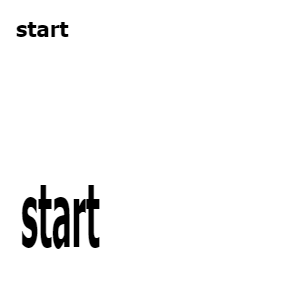
\includegraphics[width=5cm]{ss_html/canvas_scale.png}
\end{figure}

\textit{Nota}: si escala una figura, las futuras figuras estarán escaladas también.


\subsubsection{SVG vs Canvas}
\hspace{0.55cm}La \textit{Tabla \ref{tab: 1}} compara las características de ambos métodos para dibujar figuras en documentos HTML:
\begin{table}[H]
    \begin{center}
        \caption{Comparación entre Canvas y SVG}
        \label{tab: 1}
        \begin{tabular}{m{7cm} m{7cm}}
            \hline
            \textbf{Canvas} & \textbf{SVG} \\
            \hline
            \begin{enumerate}
                \item Las figuras se dibujan por programación.
                \item El dibujo es por medio de píxeles.
                \item No maneja animaciones.
                \item Excelente rendimiento para figuras dibujadas con píxeles.
                \item Dependiente de la resolución.
                \item Sin manejadores de eventos.
                \item Las figuras creadas se pueden guardar en formato \textit{.png} o \textit{.jpg}.
                \item Muy adecuado para juegos con gráficos intensivos.
            \end{enumerate}
            &
            \begin{enumerate}
                \item Las figuras forman parte del DOM del sitio web.
                \item El dibujo es por medio de vectores.
                \item Maneja animaciones.
                \item Basado en sintaxis XML estándar.
                \item Independiente de la resolución.
                \item Con manejadores de eventos.
                \item No muy adecuado para juegos.
                \item Muy adecuado para aplicaciones con grandes áreas de renderizado (por ejemplo, Google Maps).
            \end{enumerate}
            \\
            \hline
        \end{tabular}
    \end{center}
\end{table}

Podemos utilizar svg y canvas en un mismo sitio o página, pero no podemos dibujar figuras canvas dentro de un svg ni viceversa.


\subsection{Formularios HTML5}
\hspace{0.55cm}La \textit{Tabla \ref{tab: 2}} contiene las etiquetas y atributos incorporados a esta versión de HTML, junto con ejemplos:
\begin{table}[H]
    \begin{center}
        \caption{Atributos y etiquetas nuevas de formularios en HTML5}
        \label{tab: 2}
        \begin{tabular}{m{2.5cm} m{7cm} m{5cm}}
            \hline
            \textbf{Atributo o etiqueta} & \textbf{Definición} & \textbf{Ejemplo} \\
            \hline
            autofocus       & Atributo que da el foco a un control cuando el sitio o página carga                                                           & \parbox{5cm}{$<$input type="text" \\ autofocus /$>$} \\
            required        & Atributo que vuelve a un control necesario para enviar el formulario                                                          & \parbox{5cm}{$<$input type="text" \\ required /$>$} \\
            autocomplete    & Atributo que permite que un control o formulario pueda ser llenado con valores que el usuario ha ingresado previamente        & \parbox{5cm}{$<$input type="text" \\ autocomplete="off" /$>$} \\
            list            & Atributo que puede convertir una caja de texto regular en un menú desplegable (con la posibilidad de escribir todavía)        & \parbox{5cm}{$<$input type="text" \\ id="cajita" \\ list="colores" /$>$} \\
            search          & Control para crear una caja de búsqueda                                                                                       & \parbox{5cm}{$<$input type="search" \\ id="buscador" \\ name="buscaitem" /$>$} \\
            datalist        & Control complemento para \textbf{search} que define una lista de pre-valores para la caja de búsqueda. El ID de la etiqueta \textit{datalist} debe ser igual al valor del atributo \textit{list} de un control para que las opciones del primero aparezcan en el segundo                                     & \parbox{5cm}{$<$datalist id="buscador"$>$ \\ $<$/datalist$>$} \\
            options         & Sub-control complemento para \textbf{select} o \textbf{datalist} que define una lista de opciones para el menú desplegable    & $<$option value="1"$>$ \\
            email           & Control para la entrada de un correo                                                                                          & \parbox{5cm}{$<$input type="email" \\ placeholder= \\ "example@example.com" /$>$} \\
            url             & Control para la entrada de una URL                                                                                            & \parbox{5cm}{$<$input type="url" \\ placeholder="example.com" /$>$} \\
            tel             & Control para la entrada de un número telefónico                                                                               & \parbox{5cm}{$<$input type="tel" \\ placeholder="123 456 7890" /$>$} \\
            \hline
        \end{tabular}
    \end{center}
\end{table}

Algunos otras \textbf{etiquetas} y \textit{atributos} que no fueron detallados son:
\begin{itemize}
    \item \textbf{color}.
    \item \textbf{date}.
    \item \textbf{datetime}.
    \item \textbf{datetime-local}.
    \item \textbf{month}.
    \item \textbf{number}.
    \item \textbf{range}.
    \item \textbf{time}.
    \item \textit{formaction}.
    \item \textit{formenctype}.
    \item \textit{formmethod}.
    \item \textit{formnovalidate}.
    \item \textit{formtarget}.
    \item \textit{height \& width}.
    \item \textit{list}.
    \item \textit{min \& max}.
    \item \textit{multiple}.
    \item \textit{patter (regexp)}.
    \item \textit{step}.
\end{itemize}